\section{bx\_baricentrator}
\label{sec:bx_baricentrator}

This module calculates the center of light (baricenter) for each cluster; the baricenter
position is useful for a first estimation of the event vertex from where to start the real
space reconstruction minimization. Only neutrino triggers are handled; clustering is required.

Several algorithms are defined:
\begin{eqnarray}
\vec{B}_Q & = & \frac{N_Q}{n_{hits}} \sum_{i = hits} \tilde{q}_i \vec{x}_i\\
\vec{B}_T & = & \frac{N_T}{n_{hits}} \sum_{i = hits} \frac {\vec{x}_i}{t_i + T_T}\\
\vec{B}_{QT} & = & \frac{N_{QT}}{n_{hits}} \sum_{i = hits} \frac {\tilde{q}_i \vec{x}_i}{t_i + T_{QT}}
\end{eqnarray}
Where $\vec{B}$ is the baricenter position, $\vec{x}_i$ is the position of the photomultiplier which
fired that hit, $\tilde{q}_i$ is the rounded charge of the hit, $t_i$ is the time of the hit (referred to the start
of the cluster) and $n_{hits}$ is the number of hits. The values $N_x$ and $T_x$ are normalization constants for the algorithm, defined as 
module parameters (see echidna.cfg).

The calculation of the center of light is done using the hits in a configurable time gate, 
which should cut off hits from reflections and other delayed processes.
In figure~\ref{fig:cluster_time_distrib} the time distribution of the hits in the clusters is shown;
this pictures comes from a source air run (run 1610). The first reflection peak is at 50ns; to select only
the primary hits the gate should start at 0 and end at about 35ns. The {\bf first\_hits\_gate}
module parameter defines the end of the gate.

\begin{figure}[h]
\begin{center}
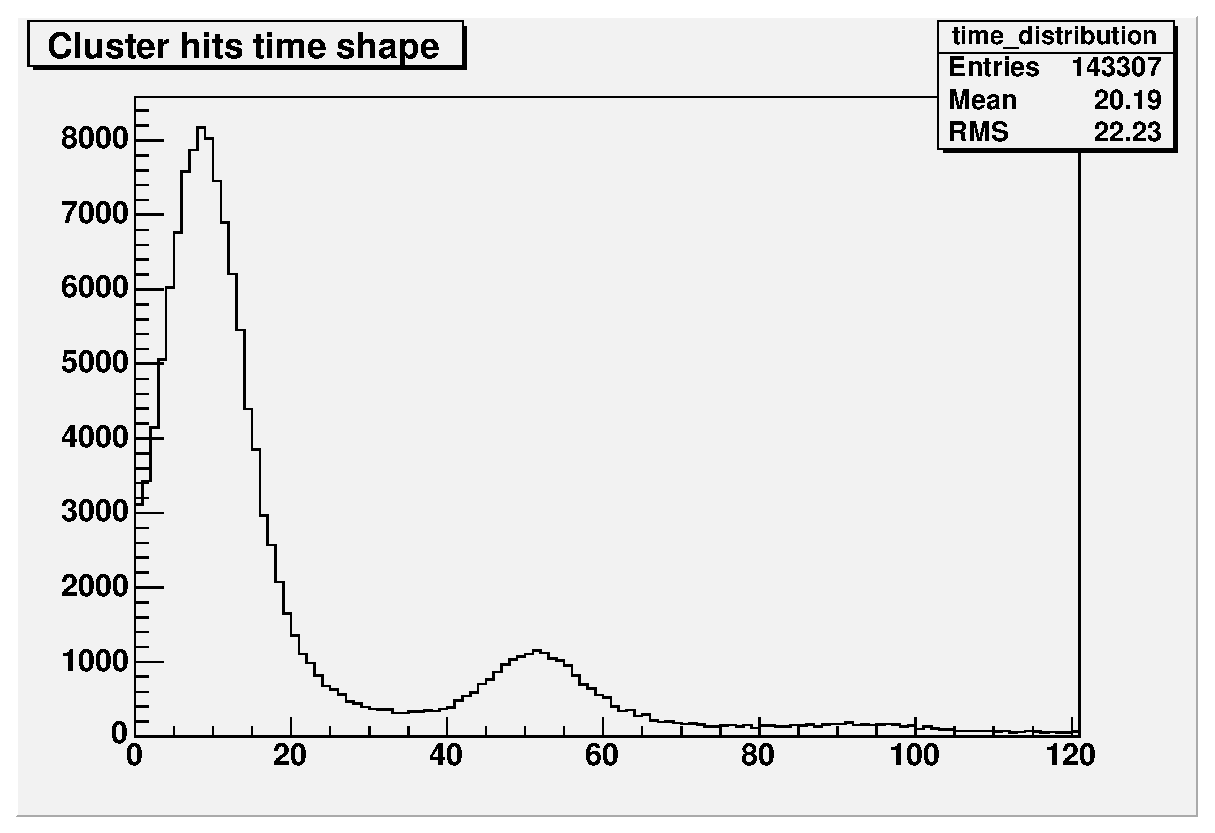
\includegraphics[width=0.8\textwidth]{pictures/cluster_time_distrib}
\caption{Cluster hits time distribution (time in ns)}
\label{fig:cluster_time_distrib}
\end{center}
\end{figure}

The $\tilde{q}_i$ is rounded to integer values starting from $q_i$ as follow: 
\[\tilde{q}_i = \left\{ \begin{array}{ll} 
0 & if\ q_i < q_0 \\
1 & if\ q_i < 0.5\ and\ q_0 < 0.5 \\
round(q_i) & else \\
\end{array}\right.\] 
where $q_0$ is defined by the module parameter {\bf zero\_charge\_limit}. The value of $n_{hits}$ is calculted
according to the algorithm and the charge ($n_{hits} = \sum_{hits} 1$ for T and $n_{hits} = \sum_{i=hits} \tilde{q}_i$ else).

\vskip 2mm
Some other values are defined as follow:
\begin{eqnarray}
\overline{t} & = & \frac{1}{n_{hits}}\sum_{i = hits}\tilde{q}_i\; t_i \\
\overline{tof} & = & \frac{1}{c\; n_{hits}} \sum_{i = hits} \tilde{q}_i\; |\vec{x}_i - \vec{B}| \\
R(t) & = & \sqrt{\frac{1}{n_{hits}}\sum_{i=hits} \tilde{q}_i \; \left[|\vec{x}_i - \vec{B}| - c(t_i + t)\right]^2} \\
t_0 & = & \overline{tof} - \overline{t}
\end{eqnarray}
Where $\tilde{q}_i$ is 1 if T algorithm is used.

$R(t)$ represents an error radius for an event with vertex in the baricenter position at time $t$;
the minimization of $R(t)$ can be done algebraically which leads to $t_{R_{min}} = t_0$. The value of
$t_0$ is a good candidate for the start time of the event and can be calculated very simply as show above.

The real vertex should be searched in the spherical volume with radius $k R_{min}$ and center in the baricenter position, 
where $k$ has to be found sperimentally.


\vskip 2mm
This module outputs the baricenter position (X, Y, Z), $R_{min}$ and $t_0$ in the laben cluster; the histograms
for $R_{min}$ is generated too.





